\DocumentMetadata{tagging=on}
\documentclass{ltx-talk}
\usepackage{tikz}
\usepackage{pdfcomment}
\tikzset{
    my callout/.style={draw,fill=blue!20!white,rectangle callout,callout absolute pointer=(pic cs:#1),below right=5pt of {pic cs:#1}},
    my callout2/.style={draw,fill=blue!20!white,rectangle callout,callout absolute pointer=(#1),below right=5pt of {#1}},
    ampersand replacement=\&,
    invisible/.style={opacity=0},
    visible on/.style={beameralt=#1{}{invisible}},
    alt/.code args={<#1>#2#3}{%
      \alt<#1>{\pgfkeysalso{#2}}{\pgfkeysalso{#3}} % \pgfkeysalso doesn't change the path
    },
    beameralt/.code args={<#1>#2#3}{%
      \alt<#1>{\pgfkeysalso{#2}}{\pgfkeysalso{#3}} % \pgfkeysalso doesn't change the path
    },
    tight matrix node/.style={draw,rectangle,inner sep=1pt, outer sep=0pt,text width=1cm,minimum height=.4cm,anchor=center},
    tight matrix node noline/.style={rectangle,inner sep=1pt, outer sep=0pt,text width=1cm,minimum height=.4cm,anchor=center},
    tight matrix/.style={
        matrix of nodes,
        inner sep=1pt, outer sep=0pt,
        row sep=-\pgflinewidth,
        column sep=-\pgflinewidth,
        nodes={tight matrix node},
    },
    tight matrix no line/.style={
        matrix of nodes,
        inner sep=1pt, outer sep=0pt,
        row sep=-\pgflinewidth,
        column sep=-\pgflinewidth,
        nodes={tight matrix node noline},
    },
}
\NewDocumentCommand\myemph{D<>{all} m}{\alert<#1>{#2}}
\newcommand{\myalttext}[2]{%
\pdftooltip{#1}{#2}%
}
\newcommand{\myalttextB}[3]{%
\only<1>{\pdftooltip{#1}{#2}}%
\only<2->{\pdftooltip{#1}{#3}}%
}

\newcommand{\myalttextC}[4]{%
\only<1>{\pdftooltip{#1}{#2}}%
\only<2>{\pdftooltip{#1}{#3}}%
\only<3->{\pdftooltip{#1}{#3}}%
}

\newcommand{\myalttextD}[5]{%
\only<1>{\pdftooltip{#1}{#2}}%
\only<2>{\pdftooltip{#1}{#3}}%
\only<3>{\pdftooltip{#1}{#3}}%
\only<4->{\pdftooltip{#1}{#4}}%
}

\begin{document}

\section{network terminology}

\subsection{nodes / links / internetworks}

\usetikzlibrary{arrows.meta,calc,shapes}
\providecommand{\computer}{%
    
\includegraphics[width=1cm]{../common/Noun_project_216.pdf}
}
\providecommand{\switch}{%
    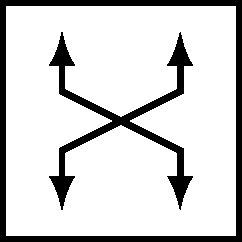
\includegraphics[width=0.9cm]{../common/fig-switch.pdf}
}
\providecommand{\router}{%
    
\includegraphics[width=0.9cm]{../common/fig-router.pdf}
}


\begin{frame}\frametitle{networks / hosts aka end systems}
\myalttextD{%
\begin{tikzpicture}
\tikzset{
    connect/.style={draw,very thick,Latex-Latex},
    computer/.style={inner sep=0mm,outer sep=0mm,beameralt=<4>{label={[font=\small,label distance=0mm,text=red]south:`host'}},execute at begin node={\computer}},
}
\node[
      cloud,draw,very thick,aspect=2,
      minimum width=4cm,minimum height=3cm,
      beameralt=<2-3>{draw=red,fill=red!10,label={[text=red]center:`network'}},
     ] (net-cloud) at (0,0) {};
\foreach \x/\d in {0/5cm,45/4cm,90/3cm,135/4cm,180/5cm,225/4cm,270/3cm,315/4cm} {
    \node[computer] (c-\x) at (\x:\d) {};
    \draw[connect] (net-cloud) -- (c-\x);
}
\coordinate (box loc) at (4cm, 3.5cm);
\tikzset{
    explain box/.style={
        overlay,draw=red, align=left, very thick, anchor=north west
    },
}
\begin{visibleenv}<2>
\node[explain box] at (box loc) {
    \textit{networks} connect \\
    computers 
};
\end{visibleenv}
\begin{visibleenv}<3>
\node[explain box] at (box loc) {
    `cloud' represents \\
    any network \\
    (whether local or not) \\
    \small iconography predates \\
    \small `cloud computing'
};
\end{visibleenv}
\begin{visibleenv}<4>
\node[explain box] at (box loc) {
    computers on edge \\
    of network called \\
    \textit{hosts} or \textit{end systems} \\
    \small (even if also `servers')
};
\end{visibleenv}
\end{tikzpicture}
}{
Picture showing computers connected via lines with arrowheads on both ends to a cloud.
}{
Same diagram as previous slide. The cloud is labeled as a `network' and a box reads ``networks connect computers''.
}{
Same diagram as previous slide. The cloud is labeled as a `network' and a box reads ``cloud represents any network (whether local or not). Iconography predates cloud computing.''
}{
Same diagram as previous slide. The computers are labeled `hosts' and a box reads ``computers on edge of network called hosts or end systems (even if also `severs').''
}
\end{frame}

\begin{frame}\frametitle{direct connections?}
\myalttext{%
\begin{tikzpicture}
\tikzset{
    connect/.style={draw,very thick,Latex-Latex},
    computer/.style={inner sep=0mm,outer sep=0mm,execute at begin node={\computer}},
}
\foreach \x/\d in {0/5cm,45/4cm,90/3cm,135/4cm,180/5cm,225/4cm,270/3cm,315/4cm} {
    \node[computer] (c-\x) at (\x:\d) {};
    \foreach \y in {0,45,90,135,180,225,270,315} {
        \ifnum \x = \y
            \relax
        \else
            \draw[connect] (c-\x) -- (c-\y);
        \fi
    }
}
\end{tikzpicture}
}{%
Picture showing 8 computers connected to each other via 56 lines (one for each pair of computers).
}
\end{frame}

\begin{frame}\frametitle{shared medium: radio?}
\myalttext{%
\begin{tikzpicture}
\tikzset{
    connect/.style={draw,very thick,Latex-Latex},
    computer/.style={inner sep=0mm,outer sep=0mm,execute at begin node={\computer}},
}
\foreach \x/\d in {0/5cm,45/4cm,90/3cm,135/4cm,180/5cm,225/4cm,270/3cm,315/4cm} {
    \node[computer] (c-\x) at (\x:\d) {};
%    %\begin{visibleenv}<2->
    \pgfmathsetmacro\oppX{\x+180}
    \path (c-\x.\oppX) -- ++(\oppX:0.1) coordinate (c-\x-wifi);
    \foreach \y in {0.2,0.35,0.5} {
        \draw[ultra thick] (c-\x-wifi) ++ (\oppX-50:\y) arc (\oppX-50:\oppX+50:\y);
    }
%    %\end{visibleenv}
}
\end{tikzpicture}
}{%
Picture showing the same 8 computers with wifi-like symbols indicating they communicate via radio.%
}
\end{frame}

\begin{frame}\frametitle{shared medium: wires}
\myalttextC{%
\begin{tikzpicture}
\tikzset{
    connect/.style={draw,very thick,arrows={Latex-Circle[width=0.3cm,length=0.3cm]},
        beameralt=<2>{arrows={Latex-Circle[width=0.3cm,length=0.3cm,red]}}},
    computer/.style={inner sep=0mm,outer sep=0mm,execute at begin node={\computer}},
}
\draw[line width=1mm] (-5,-1.5) coordinate (wire start) -- (5, 1.5) coordinate (wire end);
\foreach \x/\d in {0/5cm,45/4cm,90/3cm,135/4cm,180/5cm,225/4cm,270/3cm,315/4cm} {
    \node[computer] (c-\x) at (\x:\d) {};
    \coordinate (connect-\x) at ($(wire start)!(c-\x.center)!(wire end)$);
    \draw[connect] (c-\x) -- (connect-\x) -- ([turn]0:.1cm);
}
\begin{visibleenv}<2-3>
\node[anchor=north west,fill=white,draw=black,thick,label={[font=\tiny]south:Ali at gwc.org.uk / Alistair1978 via Wikimedia commons / CC-BY-SA 2.5}] 
    (thicknet) at (4, 3.5) {
    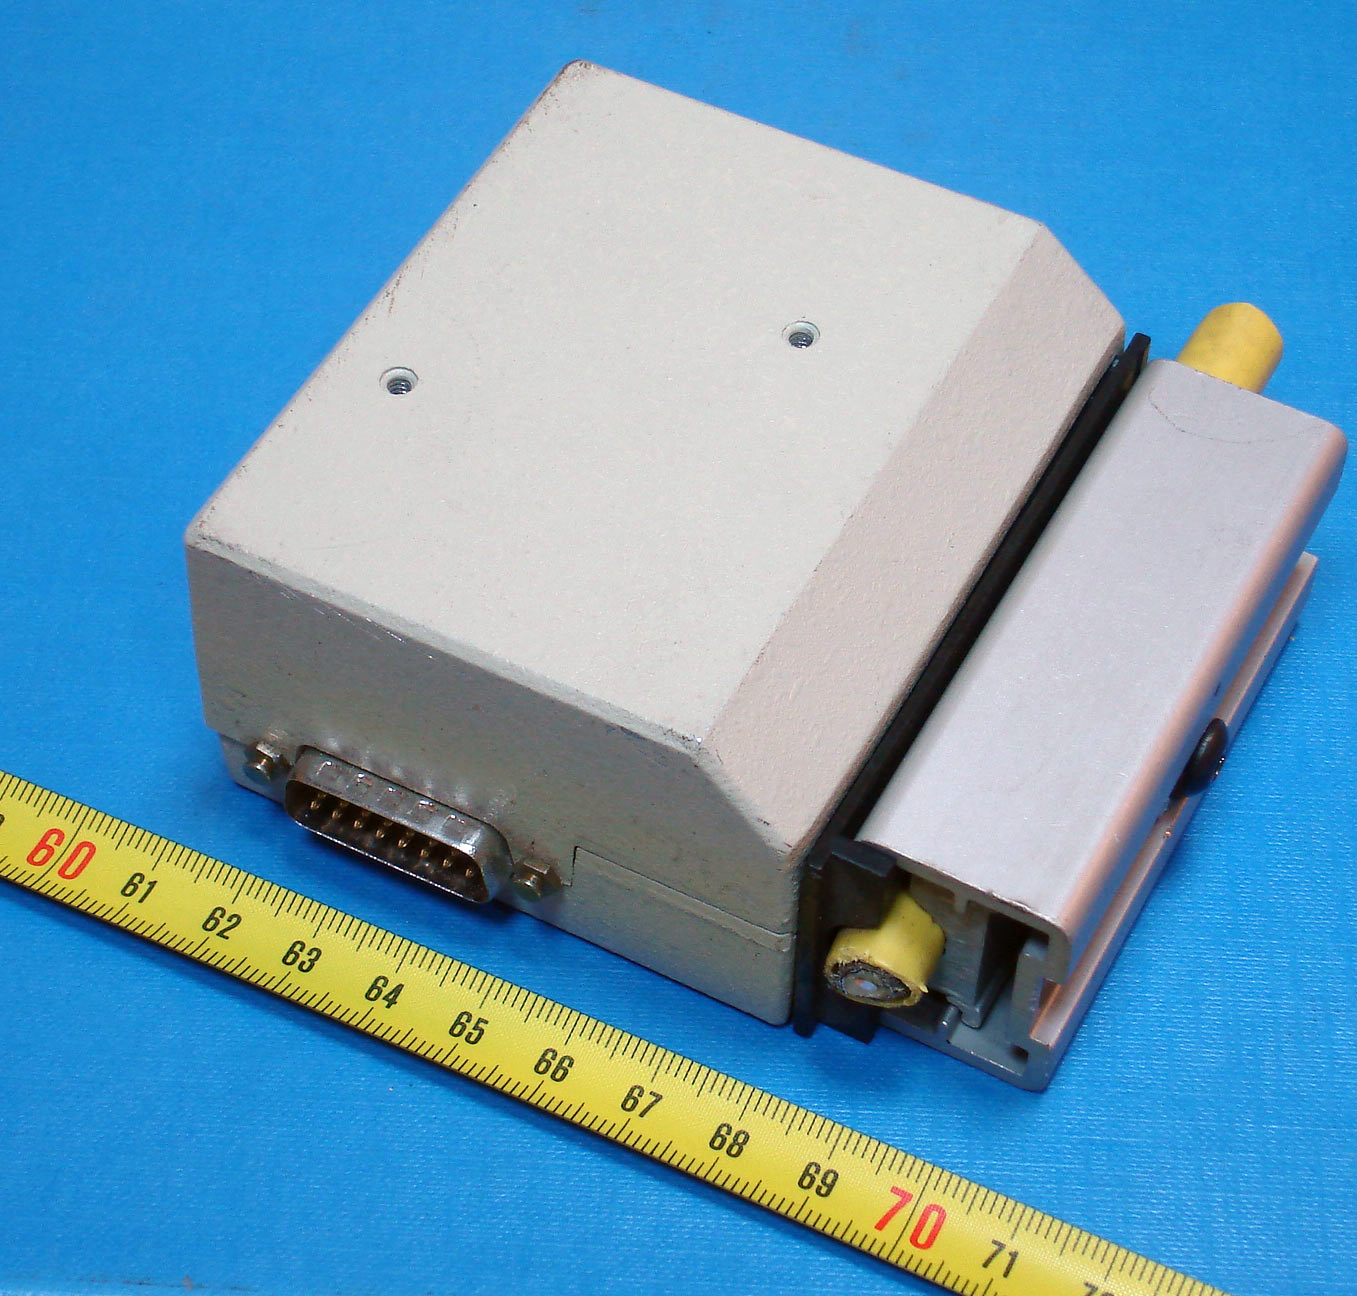
\includegraphics[width=4cm]{../intro/ThicknetTransceiver.jpeg}
};
\end{visibleenv}
\begin{visibleenv}<3>
\node[fill=white,draw=black,thick,anchor=north west] at ([yshift=-0.75cm]thicknet.south west) {
    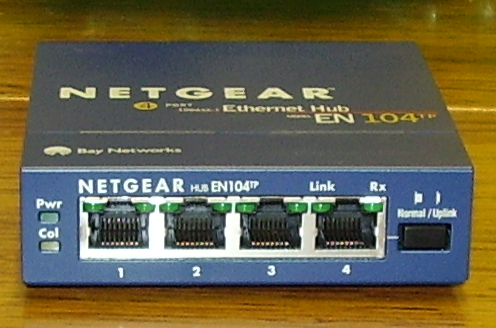
\includegraphics[width=4cm]{../intro/4_port_netgear_ethernet_hub}
};
% FIXME: also fiber splitter
\end{visibleenv}
\end{tikzpicture}
}{
Picture showing 8 computers connected via vertical lines to a single horizontal line representing a wire.
}{
Same picture as before with the connection between the vertical lines and horizontal lines highlighted, and a picture of a Thicknet transciever, a device
that screws into coax cable to provide an electrical connection.
}{
Same picture as before with the addition of a picture of a 4-port Ethernet hub --- a Netgear-branded box with four RJ-45 ports.
}
\end{frame}

\begin{frame}\frametitle{switches / nodes / links}
\begin{tikzpicture}
\tikzset{
    computer/.style={inner sep=0mm,outer sep=0mm,execute at begin node={\computer},beameralt=<3>{fill=red!10}},
    switch/.style={inner sep=0mm,outer sep=0mm,execute at begin node={\switch},
                   beameralt=<2>{
                       fill=red!10,
                        label={[font=\small,label distance=0mm,text=red]south:`switch'}
                   },
                   beameralt=<3>{fill=red!10}},
    connect/.style={draw,very thick,Latex-Latex,beameralt=<4>{red}},
    connect big/.style={draw,ultra thick,Latex-Latex,beameralt=<4>{red}},
}
\node[
      cloud,draw,opacity=0.25,very thick,aspect=2,
      minimum width=7cm,minimum height=4cm,
     ] (net-cloud) at (0,0) {};
\foreach \x/\d in {0/5cm,45/4cm,90/3cm,135/4cm,180/5cm,225/4cm,270/3cm,315/4cm} {
    \node[computer] (c-\x) at (\x:\d) {};
}
\node[switch] (s1) at (2,-0.5) {};
\node[switch] (s2) at (-1,0.5) {};
\node[switch] (s3) at (0,-1) {};
\draw[connect] (c-0) -- (s1);
\draw[connect] (c-45) -- (s1);
\draw[connect] (c-315) -- (s1);
\draw[connect] (c-90) -- (s2);
\draw[connect] (c-135) -- (s2);
\draw[connect] (c-180) -- (s2);
\draw[connect] (c-225) -- (s3);
\draw[connect] (c-270) -- (s3);
\draw[connect big] (s1) -- (s2);
\draw[connect big] (s1) -- (s3);
\coordinate (box loc) at (4cm, 4.5cm);
\begin{visibleenv}<2>
\node[overlay,draw=red, align=left, very thick, anchor=north west] at (box loc) {
    hosts directly connected to \\
    \textit{\myemph{switches}} \\
    that implement network \\
    ~ \\
    (more efficiently than \\
    shared medium)
};
\end{visibleenv}
\begin{visibleenv}<3>
\node[overlay,draw=red, align=left, very thick, anchor=north west] at (box loc) {
    machines on network \\
    (hosts, switches, \ldots) \\
    called \textit{\myemph{nodes}}
};
\end{visibleenv}
\begin{visibleenv}<4>
\node[overlay,draw=red, align=left, very thick, anchor=north west] at (box loc) {
    nodes connected by \\
   \textit{\myemph{links}} \\
    ~ \\
    (implemented by wires \\
    or radio or \ldots)
};
\end{visibleenv}
\end{tikzpicture}
\end{frame}

% FIXME: picture of physical switch

\begin{frame}{routers / internetwork}
\begin{tikzpicture}
\tikzset{
    computer/.style={inner sep=0mm,outer sep=0mm,execute at begin node={\computer}},
    switch/.style={inner sep=0mm,outer sep=0mm,execute at begin node={\switch}},
    router/.style={inner sep=0mm,outer sep=0mm,execute at begin node={\router},circle,
        beameralt=<2>{fill=red!10}},
    connect/.style={draw,very thick,Latex-Latex},
    connect big/.style={draw,ultra thick,Latex-Latex},
}
\node[
      cloud,draw,opacity=0.25,very thick,aspect=2,
      minimum width=3cm,minimum height=2cm,
     ] (net-1) at (-1,1) {};
\node[
      cloud,draw,opacity=0.25,very thick,aspect=2,
      minimum width=3cm,minimum height=2cm,
     ] (net-2) at (3,0) {};
\node[
      cloud,draw,opacity=0.25,very thick,aspect=2,
      minimum width=3cm,minimum height=2cm,
     ] (net-3) at (-2,-4) {};
\node[
      cloud,draw,opacity=0.25,very thick,aspect=2,
      minimum width=3cm,minimum height=2cm,
     ] (net-4) at (2,-3) {};

\node[
      cloud,draw,opacity=0.25,very thick,aspect=2,
      minimum width=3cm,minimum height=2cm,
     ] (net-5) at (6,-4) {};
% FIXME: routers
\node[router] (r1) at (-2, -1.5) {};
\draw[connect big] (r1) -- (net-1);
\draw[connect big] (r1) -- (net-2);
\draw[connect big] (r1) -- (net-3);
\node[router] (r2) at (5, -2) {};
\draw[connect big] (r2) -- (net-4);
\draw[connect big] (r2) -- (net-5);
\draw[connect big] (r2) -- (net-2);
\node[router] (r3) at (3, -5) {};
\draw[connect big] (r3) -- (net-3);
\draw[connect big] (r3) -- (net-5);
\coordinate (box loc) at (6, 2);
\tikzset{
    explain box/.style={
        overlay,draw=red, align=left, very thick, anchor=north west
    },
}
\begin{visibleenv}<2>
\node[explain box] at (box loc) {
    \textit{\myemph{routers}} or \textit{\myemph{gateways}} \\
    connect networks
};
\end{visibleenv}
\begin{visibleenv}<3>
\node[explain box] at (box loc) {
    connected networks \\
    form \textit{\myemph{internetwork}}
    ~ \\
    (example: the Internet)
};
\end{visibleenv}
\end{tikzpicture}
\end{frame}



\subsection{flows}

\usetikzlibrary{arrows.meta,calc,patterns,shapes}
\providecommand{\computer}{%
    
\includegraphics[width=1cm,alt={computer}]{../common/Noun_project_216.pdf}
}
\providecommand{\switch}{%
    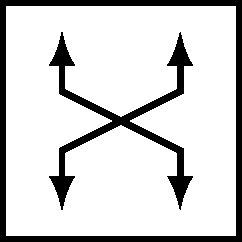
\includegraphics[width=0.9cm,alt={switch}]{../common/fig-switch.pdf}
}
\providecommand{\bigswitch}{%
    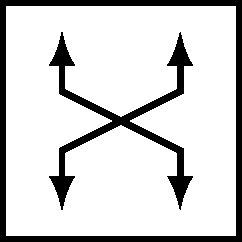
\includegraphics[width=1.4cm,alt={switch}]{../common/fig-switch.pdf}
}
\providecommand{\router}{%
    
\includegraphics[width=0.9cm,alt={router}]{../common/fig-router.pdf}
}



\begin{frame}\frametitle{flows / packets}
\begin{tikzpicture}
\tikzset{
    connect one/.style={draw,very thick,-Latex},
    computer/.style={inner sep=0mm,outer sep=0mm,execute at begin node={\computer}},
    switch/.style={inner sep=0mm,outer sep=0mm,execute at begin node={\switch}},
    big switch/.style={inner sep=0mm,outer sep=0mm,execute at begin node={\bigswitch}},
    packet/.style={minimum width=.4cm,minimum height=0.2cm,inner sep=0mm,outer sep=0mm,draw},
    packet lg/.style={minimum width=.6cm,minimum height=0.2cm,inner sep=0mm,outer sep=0mm,draw},
    c1c2/.style={fill=violet!40,draw=black,thin,slidealt=<2>{thick,draw=red}},
}
\node[computer] (c1) at (-5, 1) {};
\node at (c1) {1};
\node[big switch] (s1) at (-2,-.5) {};
\node[big switch] (s2) at (2,.5) {};
\node[computer] (c2) at (6, 2) {};
\node at (c2) {2};
\draw[connect one] (c1) -- (s1)
    node[above=0.05cm,sloped,packet,c1c2,pos=0.1] {}
    node[above=0.05cm,sloped,packet lg,c1c2,pos=0.5] {}
    node[above=0.05cm,sloped,packet,c1c2,pos=0.8] {};
\draw[connect one] (s1) -- (s2)
    node[above=0.05cm,sloped,packet,c1c2,pos=0.3] {}
    node[above=0.05cm,sloped,packet,c1c2,pos=0.8] {};
\draw[connect one] (s2) -- (c2)
    node[above=0.05cm,sloped,packet,c1c2,pos=0.2] {}
    node[above=0.05cm,sloped,packet lg,c1c2,pos=0.6] {};
\node[packet,c1c2,anchor=north east] at ([yshift=-.1cm,xshift=-.1cm]s1.north east) {};
\node[packet lg,c1c2,anchor=north east] at ([yshift=-.3cm,xshift=-.1cm]s1.north east) {};
%
\node[packet,c1c2,anchor=north east] at ([yshift=-.1cm,xshift=-.1cm]s2.north east) {};
\node[packet,c1c2,anchor=north east] at ([yshift=-.3cm,xshift=-.1cm]s2.north east) {};
\node[packet,c1c2,anchor=north east] at ([yshift=-.5cm,xshift=-.1cm]s2.north east) {};
\coordinate (box loc) at (-4, -1.5);
\tikzset{
    explain box/.style={
        overlay,draw=red, align=left, very thick, anchor=north west,at=(box loc)
    },
}
\begin{visibleenv}<1>
\node[explain box] {
    \textit{\myemph{flow}} of data between two machines \\
    ~ \\
    \textit{flow} is very general term \\
    will depend on context how it relates to \\
    connections, sockets, etc.
};
\end{visibleenv}
\begin{visibleenv}<2>
\node[explain box] {
    \textit{\myemph{flow}} of data between two machines \\
    ~ \\
    possibly divided up into pieces, \\
    called \textit{\myemph{packets}}, \textit{\myemph{frames}}, \textit{\myemph{segments}} \\
    (which name is best depends on context)
};
\end{visibleenv}
\end{tikzpicture}
\end{frame}

\begin{frame}\frametitle{(de)multiplexing}
\begin{tikzpicture}
\tikzset{%
    connect one/.style={draw,very thick,-Latex},
    connect one lg/.style={draw,line width=1mm,-Latex},
    connect one sm/.style={draw,thick,-Latex},
    computer/.style={inner sep=0mm,outer sep=0mm,execute at begin node={\computer}},
    switch/.style={inner sep=0mm,outer sep=0mm,execute at begin node={\switch}},
    big switch/.style={inner sep=0mm,outer sep=0mm,execute at begin node={\bigswitch}},
    packet/.style={minimum width=.4cm,minimum height=0.2cm,inner sep=0mm,outer sep=0mm,draw},
    packet lg/.style={minimum width=.6cm,minimum height=0.2cm,inner sep=0mm,outer sep=0mm,draw},
    c1c2/.style={fill=violet!40,draw=black,thin},
    c3c4/.style={pattern=checkerboard,pattern color=green!70,draw=black,thin},
    buffer 1/.style={slidealt=<5>{draw=red,thick},slidealt=<8>{draw=red,thick}},
    buffer 2/.style={slidealt=<5>{draw=red,thick}},
}
\node[computer] (c1) at (-5, 1) {};
\node at (c1) {1};
\node[big switch,slidealt=<3-4>{fill=red!10},slidealt=<6>{fill=red!10}] (s1) at (-2,-.5) {};
\node[big switch,slidealt=<3-4>{fill=red!10}] (s2) at (2,.5) {};
\node[computer] (c2) at (6, 2) {};
\node at (c2) {2};
\node[computer] (c3) at (-5, -1) {};
\node at (c3) {3};
\node[computer] (c4) at (6, 0) {};
\node at (c4) {4};
\draw[connect one] (c3) -- (s1)
    node[above=0.05cm,sloped,packet lg,c3c4,pos=0.2] {}
    node[above=0.05cm,sloped,packet,c3c4,pos=0.7] {};
\draw[connect one] (c1) -- (s1)
    node[above=0.05cm,sloped,packet,c1c2,pos=0.1] {}
    node[above=0.05cm,sloped,packet lg,c1c2,pos=0.5] {}
    node[above=0.05cm,sloped,packet,c1c2,pos=0.8] {};
\draw[connect one,slidealt={<2>{draw=red,ultra thick}}] (s1) -- (s2)
    node[above=0.05cm,sloped,packet,c1c2,pos=0.3] {}
    node[above=0.05cm,sloped,packet,c3c4,pos=0.6] {}
    node[above=0.05cm,sloped,packet,c1c2,pos=0.8] {};
\draw[connect one sm] (s2.north east) -- (c2)
    node[above=0.05cm,sloped,packet,c1c2,pos=0.2] {}
    node[above=0.05cm,sloped,packet lg,c1c2,pos=0.6] {};
\draw[connect one sm] (s2.south east) -- (c4)
    node[above=0.05cm,sloped,packet,c3c4,pos=0.2] {}
    node[above=0.05cm,sloped,packet lg,c3c4,pos=0.6] {};
\node[packet,c3c4,buffer 1,anchor=north east] at ([yshift=-.1cm,xshift=-.1cm]s1.north east) {};
\node[packet,c1c2,buffer 1,anchor=north east] at ([yshift=-.3cm,xshift=-.1cm]s1.north east) {};
\node[packet lg,c1c2,buffer 1,anchor=north east] at ([yshift=-.5cm,xshift=-.1cm]s1.north east) {};
\begin{visibleenv}<8>
\node[packet,c3c4,buffer 1,anchor=north east,opacity=0.9,draw=red] at ([yshift=-.7cm,xshift=-.1cm]s1.north east) {};
\node[packet lg,c1c2,buffer 1,anchor=north east,opacity=0.8,draw=red] at ([yshift=-.9cm,xshift=-.1cm]s1.north east) {};
\node[packet,c1c2,buffer 1,anchor=north east,opacity=0.7,draw=red] at ([yshift=-1.1cm,xshift=-.1cm]s1.north east) {};
\node[packet,c1c2,buffer 1,anchor=north east,opacity=0.5,draw=red] at ([yshift=-1.3cm,xshift=-.1cm]s1.north east) {};
\node[packet,c1c2,buffer 1,anchor=north east,opacity=0.3,draw=red] at ([yshift=-1.3cm,xshift=-.1cm]s1.north east) {};
\node[packet,c1c2,buffer 1,anchor=north east,opacity=0.1,draw=red] at ([yshift=-1.5cm,xshift=-.1cm]s1.north east) {};
\end{visibleenv}
\node[packet,c1c2,buffer 2,anchor=north east] at ([yshift=-.1cm,xshift=-.1cm]s2.north east) {};
\node[packet,c1c2,buffer 2,anchor=north east] at ([yshift=-.3cm,xshift=-.1cm]s2.north east) {};
\node[packet,c1c2,buffer 2,anchor=north east] at ([yshift=-.5cm,xshift=-.1cm]s2.north east) {};
\node[packet lg,c3c4,buffer 2,anchor=south east] at ([yshift=.1cm,xshift=-.1cm]s2.south east) {};
\coordinate (box loc) at (-4, -1.5);
\tikzset{%
    explain box/.style={%
        overlay,draw=red, align=left, very thick, anchor=north west,at=(box loc)
    },
}
\begin{visibleenv}<2>
\node[explain box] {%
    two or more flows can \\
    share one or more links
};
\end{visibleenv}
\begin{visibleenv}<3>
\node[explain box] {%
    left switch \textit{\myemph{multiplexes}} the two flows onto one link \\
    right switch \textit{\myemph{demultiplexes}} them to separate them
};
\end{visibleenv}
\begin{visibleenv}<4>
\node[explain box] {%
    this picture: multiplexed by dividing up \textit{time} on link
};
\end{visibleenv}
\begin{visibleenv}<5>
\node[explain box] {%
    switches usually have \textit{\myemph{buffers}} (also called \textit{\myemph{queues}}) \\
    hold waiting packets \\
    ~ \\
    absorbs temporary ``bursts'' where packets come faster \\
    than outgoing link can handle
        % FIXME: diagram of packets coming in over time
};
\end{visibleenv}
\begin{visibleenv}<6-7>
\node[explain box] {%
    incomplete list of causes of `bursts': \\
    ~ \\
    \myemph<6>{multiple unsynchronized flows} \\
    \myemph<7>{fast links produce packets faster for slow can send}
};
\end{visibleenv}
\begin{visibleenv}<8>
\node[explain box] {%
    if buffer full, switch must \textit{\myemph{drop}} packets \\
    will happen eventually if overall rate faster than outgoing link \\
    ~\\
    scenario is called \textit{\myemph{congestion}}
};
\end{visibleenv}
\end{tikzpicture}
\end{frame}

\begin{frame}\frametitle{buffer usage: fast to slow, store + forward}
\begin{tikzpicture}
\tikzset{
    axis/.style={draw,thick,-Latex},
    scale mark/.style={draw,thin},
    scale label/.style={font=\small},
    packet/.style={ultra thick,fill=violet!20},
    y=.6cm
}
\begin{scope} % input
    \begin{scope}[shift={(0.1, 0)}]
        \clip (0, 0) rectangle (12.5, 3.2);
        \draw[packet] (0, 0) coordinate (A recv start) rectangle (2, 3) node[midway] {packet A};
        \draw[packet] (2, 0) rectangle (4, 3) node[midway] {packet B};
        \draw[packet] (4, 0) rectangle (6, 3) node[midway] {packet C};
        \draw[packet] (10, 0) rectangle (12, 3) node[midway] {packet D};
    \end{scope}
    \draw[axis] (0, 0) -- ++ (12.5, 0);
    \draw[axis] (0, 0) -- ++ (0, 3.3)
        node[midway,left=.5cm,align=right] { input };
    \draw[scale mark] (0, 3) -- ++ (.25, 0) node[pos=0,left,scale label] {capacity};
\end{scope} 
\begin{scope}[shift={(0, -5)}]% buffer usage
    \begin{scope}
        \clip (0,0) rectangle (12.5, 4);
        \draw[violet, ultra thick] (0, 0) -- (0.1, 0) -- (0.1, 1) -- (2.1, 1) -- (2.1, 2) -- (4.1, 2) -- (4.1, 3)
            -- (5.1, 3) -- (5.1, 2) -- (8.1, 2) -- (8.1, 1) -- (10.1, 1) -- (10.1, 2) -- 
            (11.1, 2) -- (11.1, 1) -- (14, 1);
    \end{scope}
    \draw[axis] (0, 0) -- ++ (12.5, 0);
    \draw[axis] (0, 0) -- ++ (0, 4.3)
    node[midway,left=.5cm,align=right] (usage label) { buffer \\ reserved };
    \node[font=\small,anchor=north,align=center] at (usage label.south) {
        packets
    };
    \draw[scale mark] (0, 1) -- ++ (.25, 0) node[pos=0,left,scale label] {1};
    \draw[scale mark] (0, 2) -- ++ (.25, 0) node[pos=0,left,scale label] {2};
    \draw[scale mark] (0, 3) -- ++ (.25, 0) node[pos=0,left,scale label] {3};
    \draw[scale mark] (0, 4) -- ++ (.25, 0) node[pos=0,left,scale label] {4};

\end{scope}
\begin{scope}[shift={(0, -8)}] % output
    \begin{scope}
        \clip (0, 0) rectangle (12.5, 2.2);
        \begin{scope}[shift={(2.1, 0)}]
            \draw[packet] (0, 0) coordinate (A send start) rectangle (3, 2) node[midway] {packet A};
            \draw[packet] (3, 0) rectangle (6, 2) node[midway] {packet B};
            \draw[packet] (6, 0) rectangle (9, 2) node[midway] {packet C};
            \draw[packet] (10, 0) rectangle (13, 2) node[midway] {packet D};
        \end{scope}
    \end{scope}
    \draw[axis] (0, 0) -- ++ (12.5, 0);
    \draw[axis] (0, 0) -- ++ (0, 2.3)
        node[midway,left=.5cm,align=right] { output };
    \draw[scale mark] (0, 2) -- ++ (.25, 0) node[pos=0,left,scale label] {capacity};
\end{scope}
\begin{visibleenv}<2>
    \draw[draw=red,dotted,ultra thick,Latex-Latex] (A send start) -- ++(-2cm, 0);
    \draw[draw=red,dotted,ultra thick] (A send start) -- ++(0cm, 6cm);
    \draw[draw=red,dotted,ultra thick] ([xshift=-2cm]A send start) -- ++(0cm, 6cm);
    \node[draw=red,ultra thick,align=left,fill=white,anchor=west] at  (2.2, -3) {
        \textit{store and forward} \\
        switch stores whole packet in buffer\\
        then sends it out \\
        ~ \\
        our default in this class
    };
\end{visibleenv}
\end{tikzpicture}
\end{frame}

\begin{frame}\frametitle{buffer usage: fast to slow, cut-through}
\begin{tikzpicture}
\tikzset{
    axis/.style={draw,thick,-Latex},
    scale mark/.style={draw,thin},
    scale label/.style={font=\small},
    packet/.style={ultra thick,fill=violet!20},
    y=.6cm
}
\begin{scope} % input
    \begin{scope}[shift={(0.1, 0)}]
        \clip (0, 0) rectangle (12.5, 3.2);
        \draw[packet] (0, 0) coordinate (A recv start) rectangle (2, 3) node[midway] {packet A};
        \draw[packet] (2, 0) rectangle (4, 3) node[midway] {packet B};
        \draw[packet] (4, 0) rectangle (6, 3) node[midway] {packet C};
        \draw[packet] (10, 0) rectangle (12, 3) node[midway] {packet D};
    \end{scope}
    \draw[axis] (0, 0) -- ++ (12.5, 0);
    \draw[axis] (0, 0) -- ++ (0, 3.3)
        node[midway,left=.5cm,align=right] { input };
    \draw[scale mark] (0, 3) -- ++ (.25, 0) node[pos=0,left,scale label] {capacity};
\end{scope} 
\begin{scope}[shift={(0, -5)}]% buffer usage
    \begin{scope}
        \clip (0,0) rectangle (12.5, 4);
        \draw[violet, ultra thick] (0, 0) -- (0.1, 0) -- (0.1, 1) -- (2.1, 1) -- (2.1, 2) -- 
            (3.6, 2) -- (3.6, 1) -- (4.1, 1) -- (4.1, 2) -- (6.6, 2) -- (6.6, 1) --
            (9.6, 1) -- (9.6, 0) -- (10.1, 0) -- (10.1, 1) -- (13.6, 1) -- (13.6, 0);
    \end{scope}
    \draw[axis] (0, 0) -- ++ (12.5, 0);
    \draw[axis] (0, 0) -- ++ (0, 4.3)
    node[midway,left=.5cm,align=right] (usage label) { buffer \\ reserved };
    \node[font=\small,anchor=north,align=center] at (usage label.south) {
        packets
    };
    \draw[scale mark] (0, 1) -- ++ (.25, 0) node[pos=0,left,scale label] {1};
    \draw[scale mark] (0, 2) -- ++ (.25, 0) node[pos=0,left,scale label] {2};
    \draw[scale mark] (0, 3) -- ++ (.25, 0) node[pos=0,left,scale label] {3};
    \draw[scale mark] (0, 4) -- ++ (.25, 0) node[pos=0,left,scale label] {4};

\end{scope}
\begin{scope}[shift={(0, -8)}] % output
    \begin{scope}
        \clip (0, 0) rectangle (12.5, 2.2);
        \begin{scope}[shift={(0.6, 0)}]
            \draw[packet] (0, 0) coordinate (A send start) rectangle (3, 2) node[midway] {packet A};
            \draw[packet] (3, 0) rectangle (6, 2) node[midway] {packet B};
            \draw[packet] (6, 0) rectangle (9, 2) node[midway] {packet C};
            \draw[packet] (10, 0) rectangle (13, 2) node[midway] {packet D};
        \end{scope}
    \end{scope}
    \draw[axis] (0, 0) -- ++ (12.5, 0);
    \draw[axis] (0, 0) -- ++ (0, 2.3)
        node[midway,left=.5cm,align=right] { output };
    \draw[scale mark] (0, 2) -- ++ (.25, 0) node[pos=0,left,scale label] {capacity};
\end{scope}
\begin{visibleenv}<1>
    \draw[draw=red,dotted,ultra thick] (A send start) -- ++(-.5cm, 0);
    \draw[draw=red,dotted,ultra thick] (A send start) -- ++(0cm, 6cm);
    \draw[draw=red,dotted,ultra thick] ([xshift=-.5cm]A send start) -- ++(0cm, 6cm);
    \node[draw=red,ultra thick,align=left,fill=white,anchor=west] at  (2.2, -3) {
        \textit{cut-through} forwarding \\
        switch sends packet out as it's being received \\
        ~ \\
        uncommon and much more complex to implement
    };
\end{visibleenv}
\end{tikzpicture}
\end{frame}
% FIXME: multiplexing at end hosts


\subsection{types of channels}

\begin{frame}\frametitle{channel abstractions}
\begin{itemize}
    \item want to avoid custom network for each application
    \item but applications have different needs
    \vspace{.5cm}
    \item $\rightarrow$ multiple application interfaces to networks
    \item common implementation of \myemph{common patterns}
\end{itemize}
\end{frame}

\begin{frame}\frametitle{some abstractions}
    \begin{itemize}
    \item \myemph<2>{stream}
        \begin{itemize}
        \item continuous stream of bytes from one program to another
        \item `connection' from one program to another
        \end{itemize}
    \item datagrams
        \begin{itemize}
        \item send small messages (\textit{datagrams})
        \item each datagram's destination independently set
        \end{itemize}
    \item remote procedure calls
        \begin{itemize}
        \item make function calls that run on remote machine
        \end{itemize}
    \item remote memory access
        \begin{itemize}
        \item read/write bytes of data in remote memory
        \end{itemize}
    \item \ldots
    \end{itemize}
\end{frame}

\begin{frame}\frametitle{focus on streams}
    \begin{itemize}
    \item this class: focus on implementing \textit{streams of bytes}
    \vspace{.5cm}
    \item why?
        \begin{itemize}
        \item most commonly used by applications on the Internet
        \item many common tasks with other abstractions
        \end{itemize}
    \end{itemize}
\end{frame}


\end{document}
